
\documentclass[12pt]{article}
% LaTeX packages and global styles
% used packages in the template
% import your package here 
\usepackage{newunicodechar}
\newunicodechar{ }{\,} % U+202F NARROW NO-BREAK SPACE
\newunicodechar{Ω}{\ensuremath{\Omega}} % U+03A9 GREEK CAPITAL LETTER OMEGA
\usepackage[utf8]{inputenc}
\usepackage{multicol}
\usepackage{xcolor}
\usepackage{subfigure}
%
\usepackage[utf8]{inputenc}
\usepackage{graphicx}
\usepackage{titlesec}
\usepackage[bookmarks,breaklinks,colorlinks=true,allcolors=blue]{hyperref}
\usepackage{listings}
\usepackage{inconsolata}
\usepackage{float}
\usepackage{eso-pic}
\usepackage[framemethod=tikz]{mdframed}

\usepackage[square,numbers]{natbib}
\AtBeginDocument{
  \renewcommand{\bibsection}{\chapter{\bibname}}
} % Bibliography in numbered chapter

\usepackage{geometry}
\usepackage{amsmath}
\usepackage{parskip}
\usepackage[official]{eurosym}
\setlength {\marginparwidth }{2cm} 
\usepackage{todonotes}
\usepackage{csquotes}

\usepackage{rotating}
\usepackage{lmodern}
\usepackage{setspace}
\usepackage{pdfpages}
\usepackage{amsmath}
\usepackage{graphicx}
\usepackage{setspace}
\usepackage{xcolor}
\usepackage{eso-pic}
\usepackage{rotating}
\usepackage{textcomp} % for \textohm

% style sheet for the thesis
% Chapter and section title format
\titleformat{\section}[block]{\normalfont\huge\bfseries}{\thesection.}{.5em}{\Huge}[{}]
% \titlespacing*{\chapter}{0pt}{-19pt}{25pt}
% \titleformat{\section}[block]{\normalfont\Large\bfseries}{\thesection.}{.5em}{\Large}


\usepackage{listings}
\usepackage{xcolor}

\definecolor{codegreen}{rgb}{0,0.6,0}
\definecolor{codegray}{rgb}{0.5,0.5,0.5}
\definecolor{codepurple}{rgb}{0.58,0,0.82}
\definecolor{backcolour}{rgb}{0.95,0.95,0.92}

\lstdefinestyle{mystyle}{
    backgroundcolor=\color{backcolour},   
    commentstyle=\color{codegreen},
    keywordstyle=\color{magenta},
    numberstyle=\tiny\color{codegray},
    stringstyle=\color{codepurple},
    basicstyle=\ttfamily\footnotesize,
    breakatwhitespace=false,         
    breaklines=true,                 
    captionpos=b,                    
    keepspaces=true,                 
    numbers=left,                    
    numbersep=5pt,                  
    showspaces=false,                
    showstringspaces=false,
    showtabs=false,                  
    tabsize=2
}
% code formatting with listing
\lstset{
  style=mystyle
}

% Margins
\geometry{
    a4paper,
    margin=2.75cm
}

% Index depth limit
\setcounter{tocdepth}{2}

% Paragraph Indentation
\setlength{\parindent}{1cm}

\renewcommand{\lstlistingname}{Code extraction}
\renewcommand*{\lstlistlistingname}{Code Excerpts Index}

\definecolor{US_red}{cmyk}{0, 1, 0.65, 0.34}
\definecolor{US_yellow}{cmyk}{0, 0.3, 0.94, 0}

\mdfdefinestyle{US_style}{backgroundcolor=US_yellow!20, font=\bfseries, hidealllines=true}

% Beginning of the document
\begin{document}
   \begin{titlepage}
\centering

% Logo
\vspace*{0.8cm}

\includegraphics[width=0.32\textwidth]{images/cedtnew.png}

\vspace{0.4cm}

{\Large\bfseries Centre for Electronic Design and Technology\par}

\vspace{0.15cm}

{\large Netaji Subhas University of Technology, New Delhi\par}

% Push title towards center
\vspace*{\fill}

{\Huge\bfseries Normal Distribution of 100 k\textohm\ Resistors\par}

\vspace{1.5cm}

{\Large\bfseries Submitted by\par}

\vspace{0.4cm}

{\large Ansh Gupta and Shubham Kumar\par}

\vspace{1cm}

{\large\bfseries Date: January 2024\par}

% Bottom spacing
\vspace*{\fill}
\end{titlepage}
\section{Synopsis}
\label{chap:introduction}
%\vspace{1cm}
This project involves recording the resistance values of 1000 resistors, each nominally rated at 100 k\textohm, and analyzing the resulting data to verify the presence of a Gaussian distribution. By measuring and plotting the resistance values, the project aims to observe how closely the distribution follows the theoretical normal distribution expected for electronic components with manufacturing tolerances. The results of the analysis are crucial for understanding the statistical nature of resistor variations and can provide insights into the consistency of production processes. The report details the methodology used for data collection, the statistical tools employed for analysis, and the conclusions drawn from comparing the actual data to the theoretical Gaussian model.



\section{Introduction}
\label{sec:data}
In the realm of electronics, resistors are fundamental components used in a wide array of applications, from simple circuits to complex electronic systems. Each resistor has a specified nominal resistance value, but due to manufacturing tolerances, the actual resistance can vary. Understanding these variations is crucial for designing reliable electronic circuits. This project investigates the distribution of resistance values within a batch of resistors, specifically focusing on 1000 resistors, each nominally rated at 100 k\textohm rated as 1/8 watt with a tolerance of 5\%.

To achieve this, we undertook a systematic approach to measure and analyze the resistors' actual resistance values. The process began with the extraction of 1000 resistors from a designated box of resistors. Each resistor was carefully measured using a precision digital Multi-meter to ensure accurate readings. These measurements were then recorded meticulously in a CSV (Comma-Separated Values) file, providing a structured format for data analysis.

The primary objective of this study was to analyze the distribution of these resistance values and assess whether they follow a Gaussian distribution, which is a common theoretical model for such variations. To visualize and evaluate the data, we employed the matplotlib library, a powerful tool for creating plots and graphs in Python. By plotting the distribution curve of the recorded resistance values, we aimed to verify the conformity of the data to the expected Gaussian distribution, providing insights into the consistency and reliability of the resistors' manufacturing process.

Through this investigation, we seek to understand the degree of variation in resistor values and assess the quality control measures in place during manufacturing. The results of this analysis have implications for electronic design, particularly in ensuring that resistors used in circuits meet the required specifications and perform reliably under different conditions.

 
\newpage
\section{Working}
\label{chap:results}
\raggedright

The steps for this experiment are very concise and straightforward. They are as follows:
\begin{itemize}
    \item \subsection{\underline{ Resistance Measurement }}
    
    
       To conduct the experiment, we began by selecting a box of resistors, from which we extracted 1000 resistors, each with a nominal value of 100 k\textohm. Using a precision digital multi-meter, we meticulously measured the resistance of each resistor. The recorded values were then compiled into a CSV file for further analysis. 

   

    
    \item \subsection{\underline{Curve Plotting}}
    To Visualize the Gaussian distribution with the measured value of resistance create the CSV file of the recorded value of resistance and plot it with the help of Python library (  Matplotlib, Pandas, Seaborn, Numpy, and Scipy.stats) which helps us to creating a smooth curve.
    
\end{itemize}
 \newpage
    

    



\newpage

\section{Observation}


\begin{figure}[H]
    \centering
    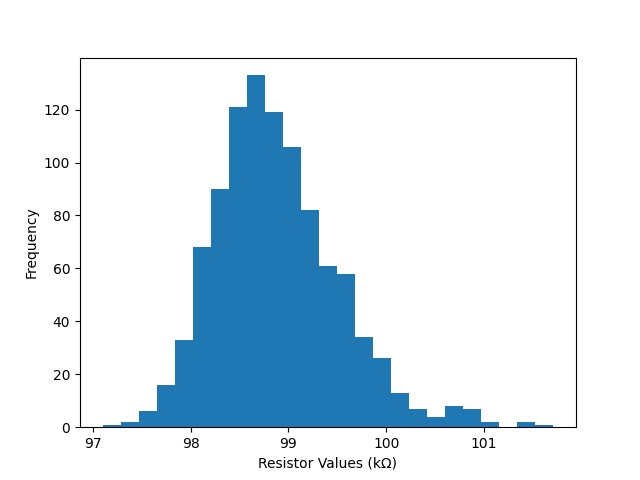
\includegraphics[width=15cm]{images/graph.jpg}
    \caption{Observed Graph of Distribution for 100K\textohm Resistor}
    \label{fig_figure1}
\end{figure}
The resistance values of 1000 resistors were measured and analyzed to examine their distribution. The histogram, as shown in Figure \ref{fig_figure1}, illustrates the spread of these measured values, centered around the nominal value of 100 k\textohm. The peak of the distribution occurs near 99 k\textohm, with values ranging between approximately 97 k\textohm and 101 k\textohm.

In this study, we aimed to observe whether the distribution of resistor values follows a typical Gaussian (normal) distribution. The shape of the histogram shows a bell curve that closely resembles a Gaussian distribution, with most resistors clustered around the mean and fewer at the extremes. While there are minor deviations from the ideal normal curve, particularly on the lower end, the overall distribution largely fulfills the requirements of a Gaussian distribution. These deviations are expected given manufacturing tolerances, confirming the consistency and reliability of the resistor batch.

\newpage
\section{Conclusion}
\begin{itemize}
\item The analysis of the resistance values measured from 1000 resistors, each with a nominal value of 100 kΩ and a tolerance of ±5\%, shows a distribution that closely aligns with a Gaussian (normal) distribution pattern.
\item Using Python libraries such as Pandas, NumPy, Seaborn, and Scipy, the histogram of the resistance values was plotted and analyzed. The central tendency of the data was found near 99 kΩ, slightly below the nominal rating, with the full data range extending from approximately 97 kΩ to 101k\textohm.
\end{itemize}

\section{Appendix}
\subsection*{Data File}

\begin{itemize}
  \item \href{https://drive.google.com/drive/folders/1Y8cfFo5tjva2JRQHohGjNMzd-atVvMah?usp=drive_link}{Resistor Values}
\end{itemize}
\vspace{-5mm}
\subsection*{Code Files}
\begin{itemize}
  \item \href{https://drive.google.com/drive/folders/13z_Cev9iF9TGuNE9fz6Ii99t_w-Qxyss?usp=drive_link}{Python Code}
\end{itemize}

    
    

\end{document}
